% Guarding Walls Contiguously -- project report
% INFO-F420 Computational Geometry, Universite libre de Bruxelles, 2026-2027
% Compile with pdfLaTeX (Overleaf: default settings). The figures are in figures/.

\documentclass[11pt,a4paper]{article}

\usepackage[T1]{fontenc}
\usepackage{lmodern}
\usepackage{microtype}
\usepackage[a4paper,margin=2.4cm]{geometry}
\usepackage{amsmath,amssymb,amsthm}
\usepackage{graphicx}
\usepackage{booktabs}
\usepackage{tabularx}
\usepackage[shortlabels]{enumitem}
\usepackage{xcolor}
\usepackage[colorlinks=true,linkcolor=blue!50!black,citecolor=blue!50!black,urlcolor=blue!50!black]{hyperref}

\graphicspath{{figures/}}
\setlist{itemsep=2pt,topsep=4pt}
\renewcommand{\arraystretch}{1.25}
\newcolumntype{Y}{>{\raggedright\arraybackslash}X}

\newtheorem{theorem}{Theorem}
\newtheorem{lemma}{Lemma}
\newtheorem{proposition}{Proposition}
\newtheorem{corollary}{Corollary}
\newtheorem{observation}{Observation}
\theoremstyle{definition}
\newtheorem{definition}{Definition}
\theoremstyle{remark}
\newtheorem*{remark}{Remark}

% the results of the paper keep the numbering of [5]
\newcommand{\paperthm}[2]{\expandafter\renewcommand\csname the#1\endcsname{#2}}
\newcommand{\nextop}{\mathrm{next}}
\newcommand{\bd}{\partial P}
\newcommand{\by}[1]{\hfill{\small\textit{(explained by #1)}}}


\title{\textbf{Guarding Walls Contiguously}\\[4pt]
\large An interactive exploration of the Contiguous Art Gallery Problem\\[2pt]
\normalsize Project report --- INFO-F420 Computational Geometry, Universit\'e libre de Bruxelles, 2026--2027}
\author{Ilias Akajou (520466) \and Jomaa Abdulrahman (583629)}
\date{November 2026}

\begin{document}
\maketitle

\begin{center}
\begin{tabular}{@{}ll@{}}
\textbf{Public webpage} & \url{https://iakajou.github.io/contiguous-art-gallery/} \\
\textbf{Source code}    & \url{https://github.com/iakajou/contiguous-art-gallery} \\
\end{tabular}
\end{center}

\begin{abstract}
In the \emph{Contiguous Art Gallery Problem}, we want to guard the boundary of a simple polygon $P$ with as few guards as possible, where each guard
watches one connected part of the boundary. Unlike almost all other art gallery problems, this one can be solved in polynomial time. Our project explains
the short proof and the $O(kn^2\log^2 n)$-time algorithm of de Berg, Conradi, van der Hoog and Staals~\cite{deBerg2025}. We built an interactive webpage that
follows the proof step by step, with one interactive figure per step, all computed live by our own JavaScript implementation of the whole algorithm.
We validated the implementation and every construction of the proof against brute-force computations, and found that the statement of one lemma
(Lemma~6.2) needs a precision when a chain winds around the guard more than once. This report summarises the problem, the proof, our implementation
and how we shared the work. The webpage contains the detailed proof.
\end{abstract}

\tableofcontents

%======================================================================
\section{Introduction}
%======================================================================

\subsection{The problem}

Let $P$ be a \emph{simple polygon} with $n$ vertices: a single closed boundary $\bd$, without self-intersections and without holes. A point $g\in P$
\emph{sees} a point $q$ if the segment $gq$ is contained in $P$ (we treat $P$ as a closed set, so a segment may touch the boundary).

\begin{definition}
A \emph{contiguous guard} is a pair $(g,[u,v])$ of a point $g\in P$ and a connected part $[u,v]$ of $\bd$, called its \emph{chain}, such that $g$ sees
every point of $[u,v]$. The \emph{Contiguous Art Gallery Problem} asks for the minimum number $k$ of contiguous guards whose chains cover $\bd$.
\end{definition}

An easy way to think about it: each guard is a security camera that turns and films one stretch of wall, without skipping anything.
We may assume that the chains do not overlap, so an optimal solution is a partition of the boundary into $k$ chains. One guard is enough if and only if $P$ is
star-shaped. Figure~\ref{fig:guard} shows the first widget of our webpage.

\begin{figure}[ht]
\centering
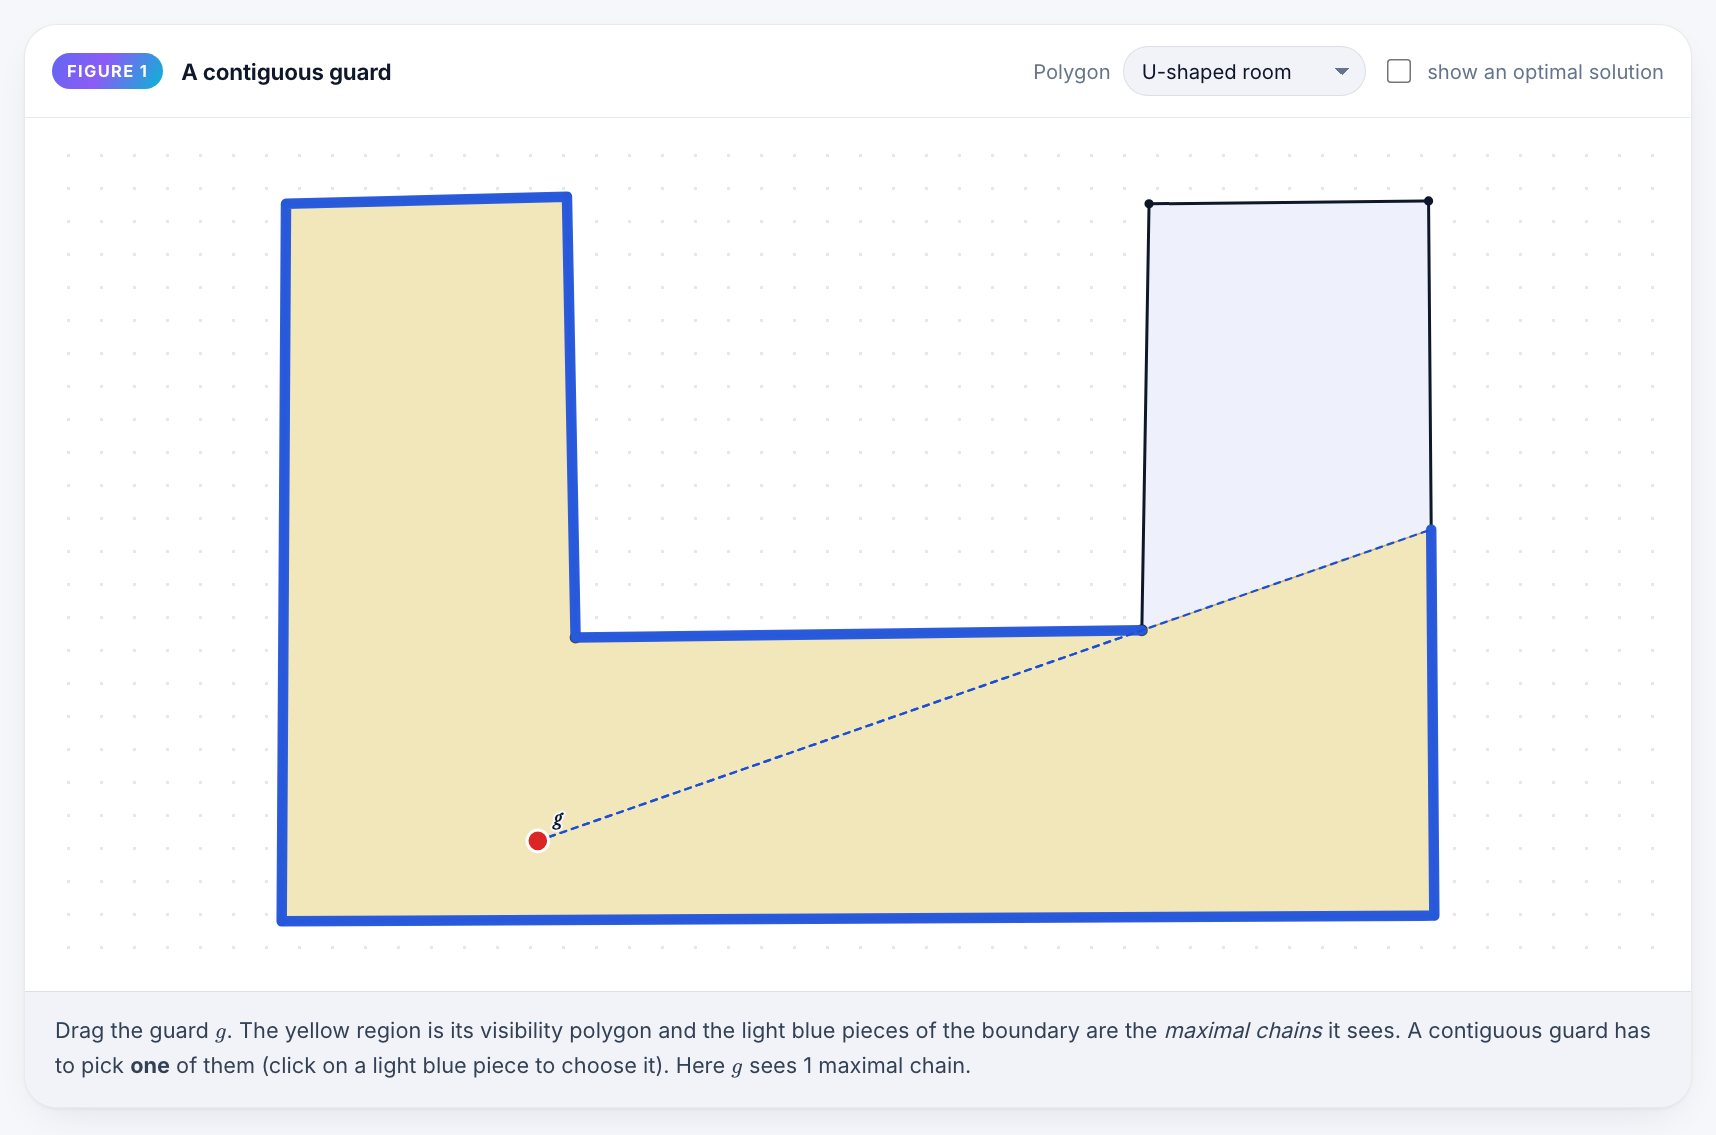
\includegraphics[width=0.78\linewidth]{fig01}
\caption{Figure 1 of our webpage. The yellow region is what the point $g$ sees; the light blue pieces of the boundary are the maximal chains it sees.
A contiguous guard keeps only one of them. The room is not star-shaped, so $k=2$.}
\label{fig:guard}
\end{figure}

\paragraph{The simple-polygon assumption is essential.} All the papers on this problem assume that $P$ is simple, and the method fails without it:
(i)~the boundary must be a single cycle, which is what the greedy argument covers with intervals; (ii)~every closed curve in $P$ encloses only points of $P$,
which all the proofs use, and shortest paths are unique; (iii)~with a hole, a guard can see both endpoints of an edge without seeing its middle.
Merrild et al.~\cite{Merrild2024} note that their approach does not extend to polygons with holes, and that the complexity of this case is open.
Our solver rejects non-simple polygons.

\subsection{Why the problem is surprising}

Most art gallery problems are hard. The classical problem (point guards that must see the whole polygon) is NP-hard~\cite{LeeLin1986} and even
$\exists\mathbb{R}$-complete~\cite{Abrahamsen2022}, and guarding only the boundary with point guards is still $\exists\mathbb{R}$-hard~\cite{Stade2025}.
Adding the contiguity constraint looks like it should make things harder, but it does the opposite: every guard covers a single interval of a
one-dimensional object, the boundary, and covering a circle with intervals is easy once we know where to start. Following the feedback on our proposal,
we do not re-explain the classical art gallery problem (Chv\'atal's $\lfloor n/3\rfloor$ theorem~\cite{Chvatal1975}), which is covered by many resources,
and focus on the algorithm of~\cite{deBerg2025}.

\subsection{Our contribution}

\begin{itemize}
\item An interactive webpage on GitHub Pages: a short overview that we use for the presentation, five chapters that follow the proof of~\cite{deBerg2025}
step by step with eleven interactive figures, a game, and the report.
\item A complete implementation of the algorithm in JavaScript, running in the browser, with simpler polynomial-time subroutines instead of the
polylogarithmic data structures of the paper.
\item Automatic tests that check the implementation and every construction of the proof against independent brute-force computations.
\item A precision on Lemma~6.2 of~\cite{deBerg2025}, found with these tests (Section~\ref{sec:lemma62}).
\end{itemize}

%======================================================================
\section{Related work}
%======================================================================

The problem was posed by T.~Shermer at the open problem session of CCCG 2024. In about one year it went from an open question to an optimal algorithm
(Table~\ref{tab:history}).

\begin{table}[ht]
\centering
\begin{tabularx}{\linewidth}{@{}l Y Y l@{}}
\toprule
Year & Reference & Main idea & Running time \\
\midrule
2024 & Shermer (CCCG open problem) & problem posed & open \\
2024--25 & \cite{Merrild2024,Biniaz2024,Robson2024} $\to$ \cite{Biniaz2025} (SoCG 2025) & repeated greedy; $O(n^4)$ candidates; analytic arc cover & $O(kn^5\log n)$ \\
\textbf{2025} & \textbf{de Berg, Conradi, van der Hoog, Staals~\cite{deBerg2025}} & \textbf{greedy from $O(n^2)$ candidate starts} & $\boldsymbol{O(kn^2\log^2 n)}$ \\
2025--26 & de Berg, Conradi, van der Hoog, Rotenberg~\cite{deBerg2026} & dominators, sliding window, M\"obius pieces & $\Theta(n\log n)$ \\
\bottomrule
\end{tabularx}
\caption{Algorithms for the Contiguous Art Gallery Problem.}
\label{tab:history}
\end{table}

\begin{itemize}
\item \textbf{One guard.} Lee and Preparata~\cite{LeePreparata1979} compute the kernel of a polygon in $O(n)$ time, which decides whether $k=1$.
\item \textbf{First polynomial algorithms.} Merrild, Rysgaard, Schou and Svenning~\cite{Merrild2024} show that the greedy algorithm uses at most $k+1$ guards,
and restart it $O(kn^3)$ times, which gives $O(kn^5\log n)$ time. Biniaz et al.~\cite{Biniaz2024} give an exact algorithm that computes $O(n^4)$ candidate guard locations and combines them;
they also show that $\lfloor (n-2)/2\rfloor$ contiguous guards always suffice. Robson, Spalding-Jamieson and Zheng~\cite{Robson2024} reduce the problem to the \emph{analytic arc cover problem}, solved with tools
from real algebraic geometry; they showed that $\nextop$ is a piecewise function with $O(n^3)$ pieces~\cite{deBerg2026}. The three works were merged at SoCG 2025~\cite{Biniaz2025}.
\item \textbf{Our paper.} De Berg, Conradi, van der Hoog and Staals~\cite{deBerg2025} show that $O(n^2)$ starting points suffice and that one greedy step
costs $O(\log^2 n)$, hence $O(kn^2\log^2 n)$. Their paper is short (12 pages including references) and almost self-contained, which is why we chose it.
\item \textbf{Optimal bound.} De Berg, Conradi, van der Hoog and Rotenberg~\cite{deBerg2026} use $O(n)$ starting points and a function $\nextop$ made of $O(n)$
M\"obius pieces, which gives $O(n\log n)$ time, with a matching $\Omega(n\log n)$ lower bound by a reduction from set disjointness.
\item \textbf{Tools.} Shortest-path queries in $O(\log n)$ after linear preprocessing (Guibas and Hershberger~\cite{GuibasHershberger1989},
Guibas et al.~\cite{Guibas1987}), and ray shooting in $O(\log n)$ (Hershberger and Suri~\cite{HershbergerSuri1995}).
\end{itemize}

%======================================================================
\section{The algorithm of de Berg et al.}
\label{sec:algo}
%======================================================================

We summarise the proof, keeping the numbering of~\cite{deBerg2025} so that it can be compared with the paper. Each step is illustrated on the webpage by
an interactive figure, and the person who explains it is indicated.

\paragraph{Notation.} The vertices $v_0,\dots,v_{n-1}$ are numbered counter-clockwise, and a point of $\bd$ is a real number $t\in[0,n)$: the integer part is
the edge, the fractional part the position on the edge. A chain $[u,v]$ is the part of $\bd$ from $u$ to $v$ counter-clockwise. For a set $E$ of edges,
the \emph{visibility core} $P_E$ is the intersection of the closed half-planes to the left of the supporting lines of the edges of $E$.

\paperthm{observation}{2.1}
\begin{observation}
If $g$ sees a chain $[u,v]$, then $g$ lies in the visibility core of the edges of $[u,v]$.
\end{observation}
\paperthm{observation}{2.2}
\begin{observation}
One guard suffices ($k=1$) if and only if $P_{\bd}$, the kernel of $P$, is not empty; this can be tested in $O(n)$ time~\cite{LeePreparata1979}.
\end{observation}

\subsection[The greedy algorithm]{The greedy algorithm \by{Ilias Akajou}}

For $u\in\bd$, let $\nextop(u)$ be the farthest point $v$ (counter-clockwise) such that some guard sees $[u,v]$. The greedy algorithm from $u$ takes the
guard that realises $\nextop(u)$, restarts from $\nextop(u)$, and stops when the chains cover $\bd$. Let $G_u$ be its result.

\paperthm{lemma}{(greedy)}
\begin{lemma}
For every $u$, $|G_u|\le k+1$. If an optimal solution has a chain that starts at $u$, then $|G_u|=k$.
\end{lemma}
\begin{proof}[Proof sketch (``the greedy stays ahead'')]
Number the chains $[u^*_i,v^*_i]$ of an optimal solution along $\bd$, starting with the chain that contains $u$ (index $0$), and let $[u_i,v_i]$ be the chains
of the greedy algorithm, with $u_1=u$ and $u_{i+1}=v_i$. By induction, $v_i\ge v^*_{i-1}$: the optimal guard $0$ sees $[u,v^*_0]$, so $v_1\ge v^*_0$; and if
$v_i\le v^*_i$, then $u_{i+1}=v_i$ lies in the optimal chain $i$, whose guard sees $[u_{i+1},v^*_i]$, so $v_{i+1}\ge v^*_i$. After $k+1$ steps the greedy
has gone around $\bd$. If $u$ is the start of an optimal chain, we number it $1$ instead of $0$ and $k$ steps suffice.
\end{proof}

So for every $u$, $k\in\{|G_u|-1,|G_u|\}$, and the whole problem is to find a good starting point. Merrild et al.\ restart the greedy $O(kn^3)$ times;
the contribution of~\cite{deBerg2025} is a set $U_P$ of only $O(n^2)$ starting points, one of which is guaranteed to start an optimal chain.

\begin{figure}[ht]
\centering
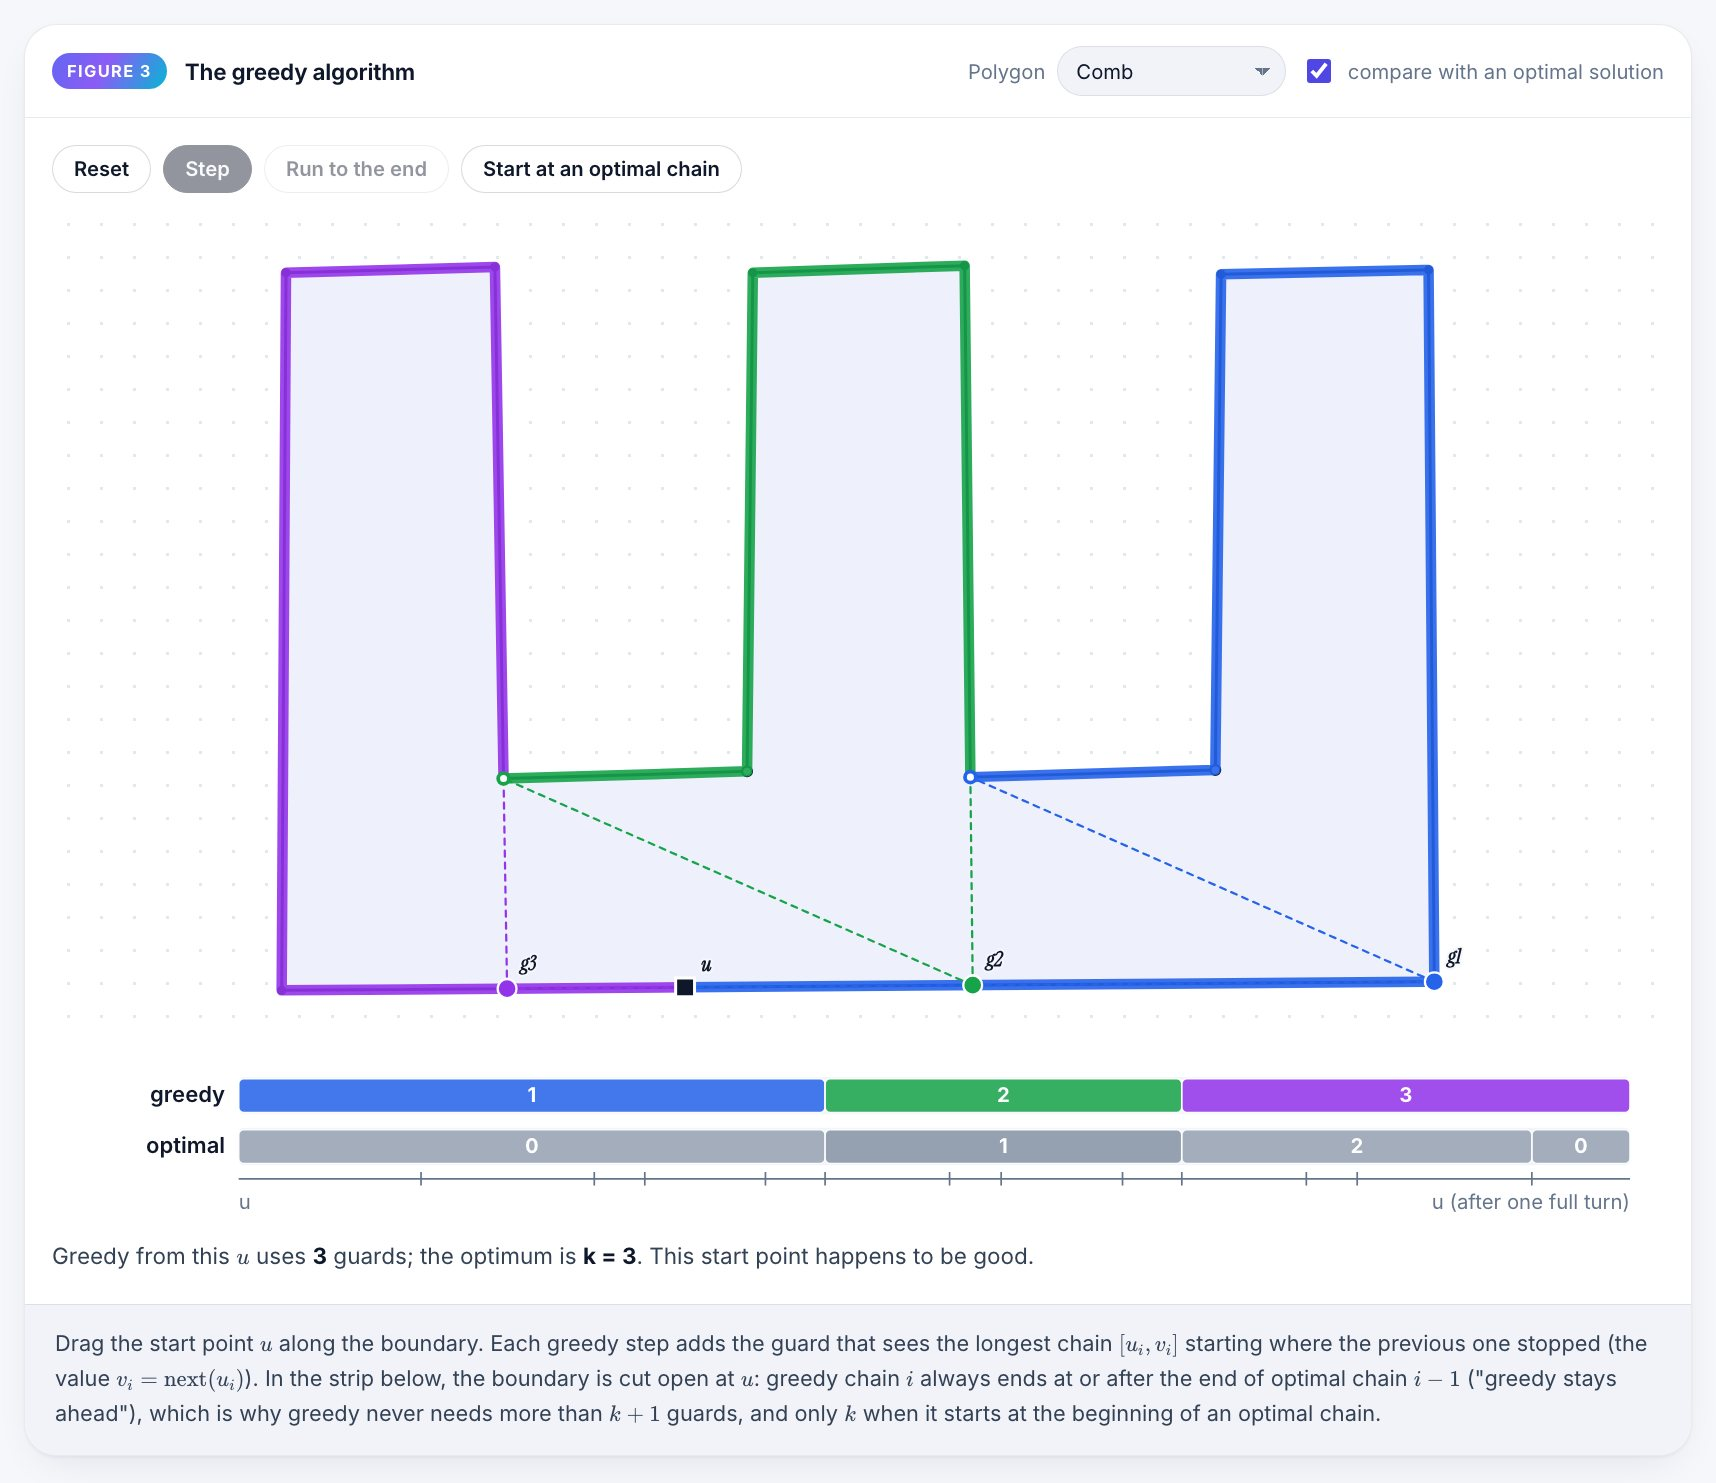
\includegraphics[width=0.66\linewidth]{fig03}
\caption{Figure 3 of our webpage: the greedy algorithm on the polygon \emph{Comb}. The strip at the bottom cuts the boundary open at the start point and
compares the greedy chains with an optimal solution: the greedy always stays ahead.}
\label{fig:greedy}
\end{figure}

\subsection[Good and bad guards]{Good and bad guards \by{Ilias Akajou}}

\paperthm{definition}{4.1}
\begin{definition}
A contiguous guard $(g,[u,v])$ is \emph{bad} if (I)~the open chain $(u,v)$ contains a vertex of $P$, (II)~$g\neq u$ and $g\neq v$,
(III)~the angle $\angle(v,g,u)$ under which $g$ sees its chain is larger than $\pi$, and (IV)~the shortest path from $u$ to $v$ in $P$ is not a single
segment. Otherwise it is \emph{good}.
\end{definition}

A good guard looks at its chain ``from the front''; a bad guard looks ``around an obstacle'' (Figure~\ref{fig:goodbad}).

\paperthm{observation}{4.8}
\begin{observation}
If $(g,[u,v])$ is bad, the shortest path from $u$ to $v$ is a convex chain that always turns left.
\end{observation}

\begin{figure}[ht]
\centering
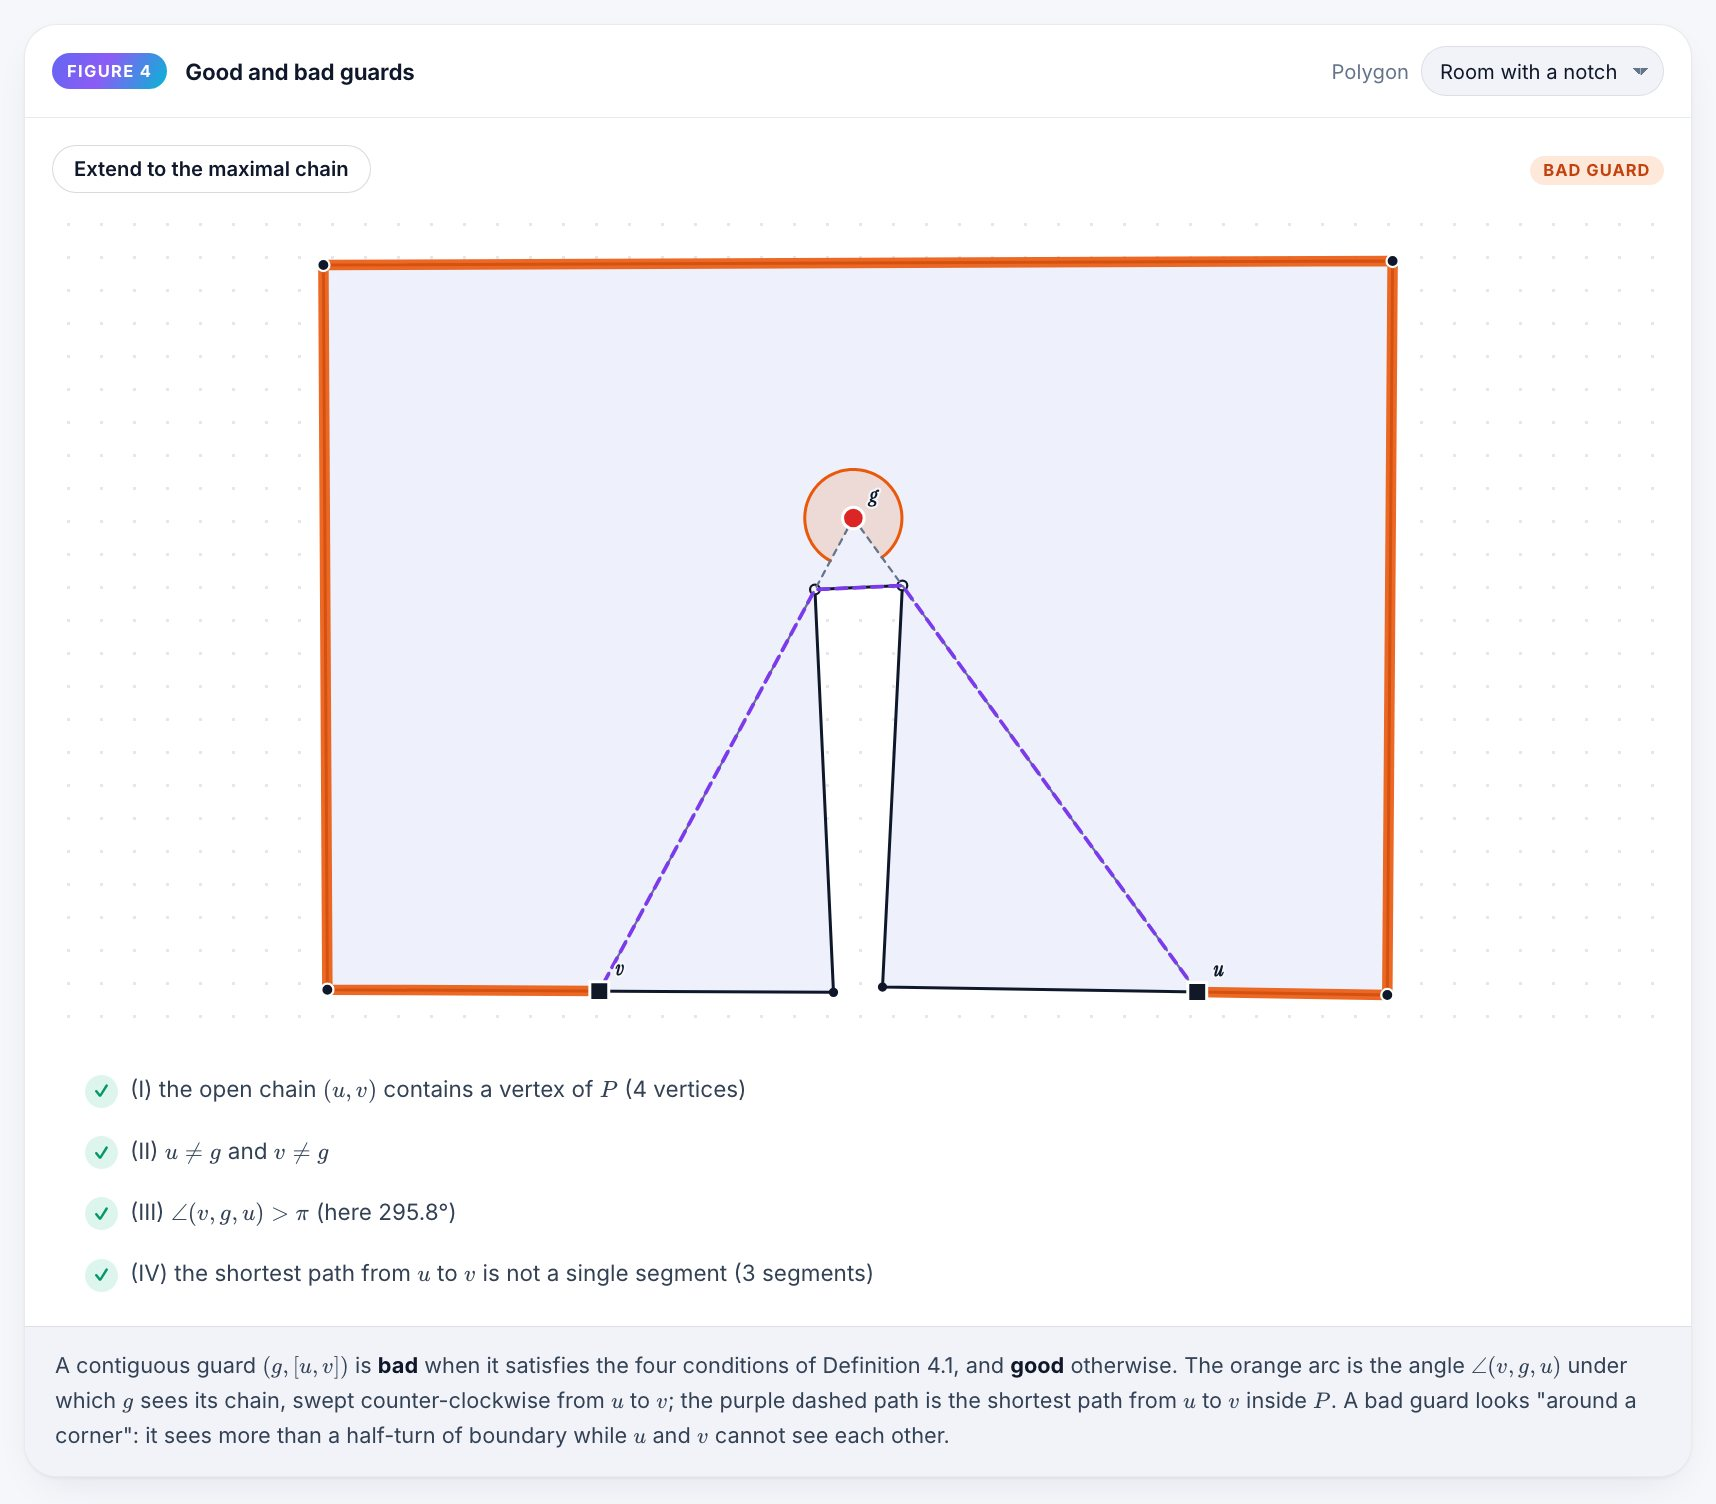
\includegraphics[width=0.48\linewidth]{fig04}\hfill
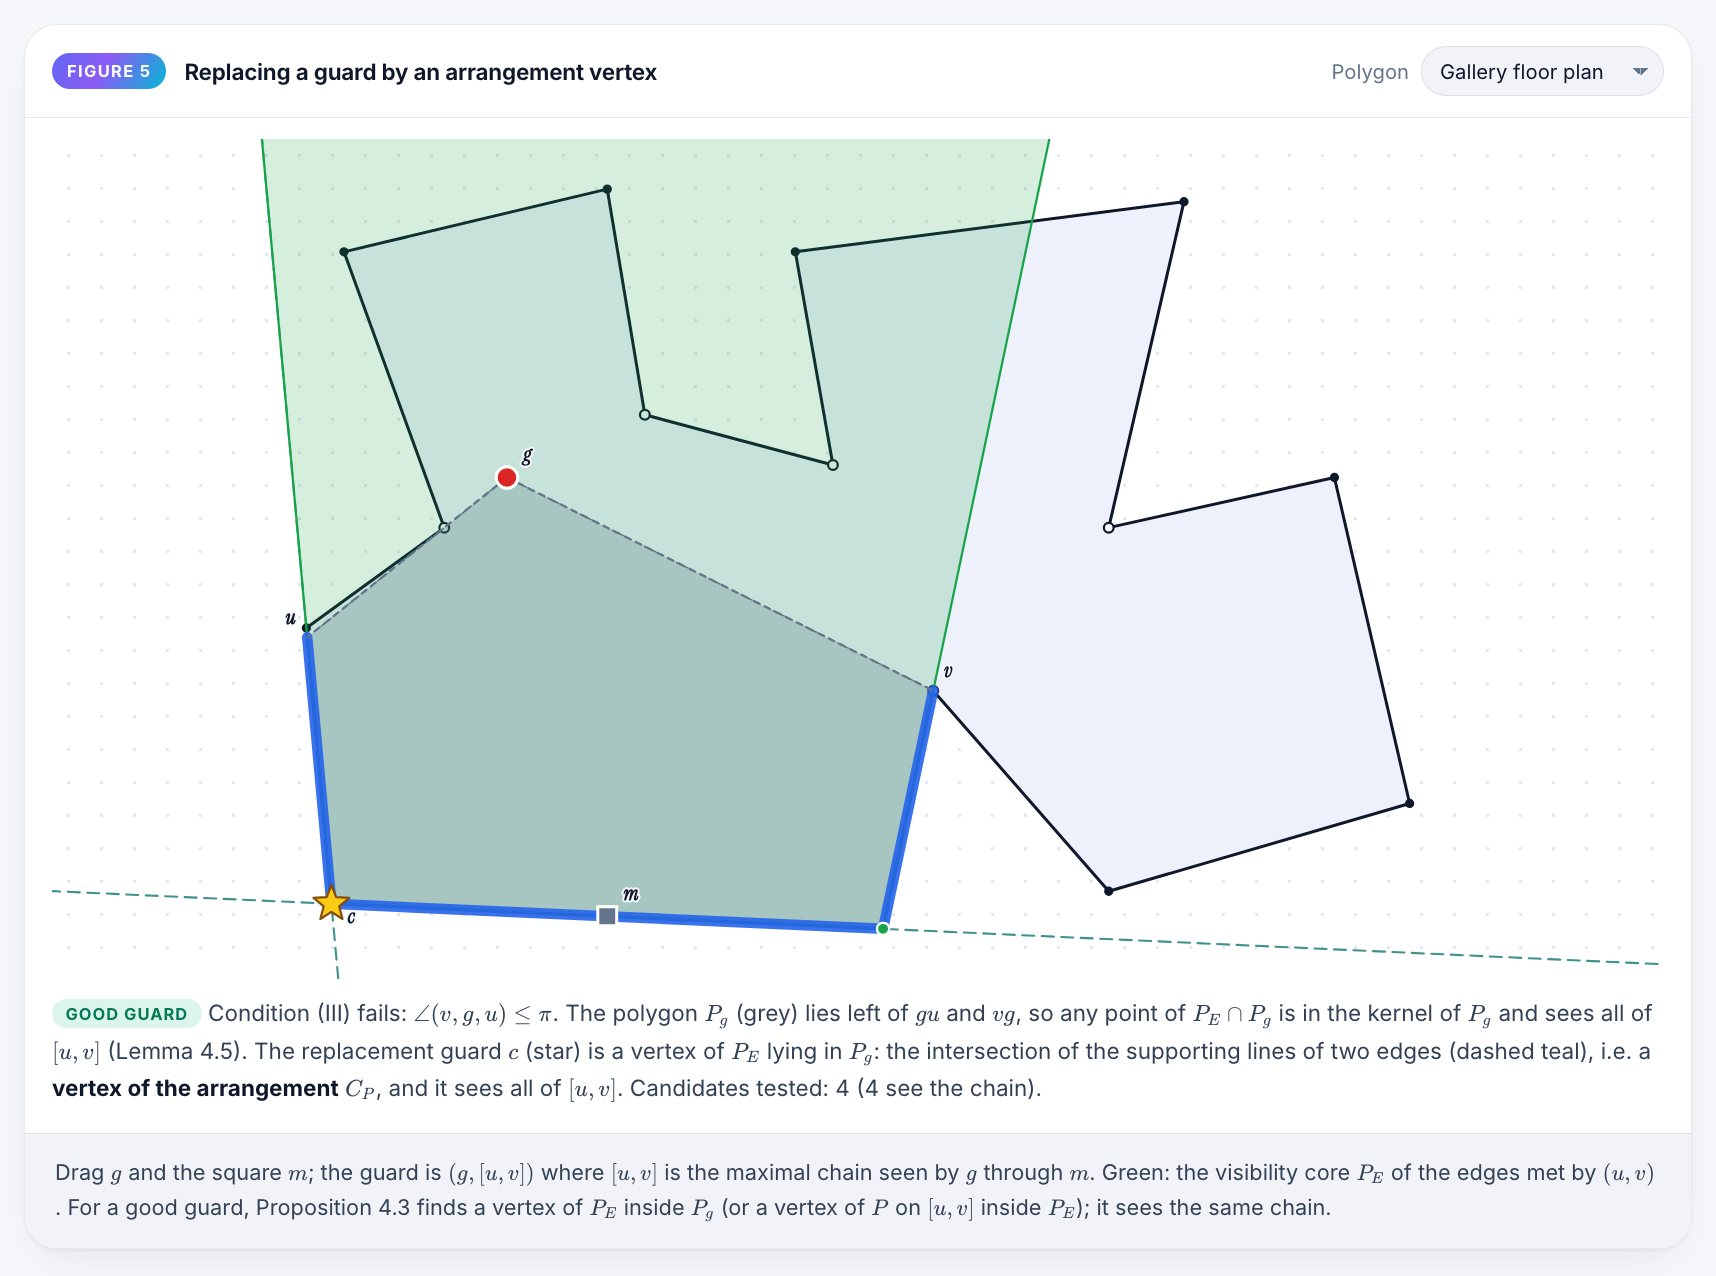
\includegraphics[width=0.48\linewidth]{fig05}
\caption{Left: Figure 4 of our webpage, a bad guard in a room with a notch; the four conditions of Definition~4.1 are evaluated live.
Right: Figure 5, a good guard (red) replaced by a vertex of the arrangement (star), which sees the same chain.}
\label{fig:goodbad}
\end{figure}

\subsection[Replacing guards]{Replacing guards \by{Ilias Akajou}}

Let $P_g$ be the polygon bounded by $gu$, the chain $[u,v]$ and $vg$, and let $P_E$ be the visibility core of the edges of the chain.

\paperthm{proposition}{4.3}
\begin{proposition}
Some vertex of $P_E$ lies in $P_g$, or some vertex of the chain $[u,v]$ lies in $P_E$.
\end{proposition}

Such a point is to the left of every edge of the chain. Each condition of Definition~4.1 that fails gives the missing argument
(Lemma~4.2: the chain lies in one edge; Lemma~4.4: $g=u$; Lemma~4.5: angle at most $\pi$; Lemma~4.6: $u$ sees $v$), and we obtain:

\paperthm{corollary}{4.7}
\begin{corollary}
Every good guard $(g,[u,v])$ can be replaced by a guard $(c,[u,v])$ where $c$ is a vertex of the arrangement $C_P$ of the supporting lines of the edges of $P$.
\end{corollary}

\paperthm{lemma}{4.9}
\begin{lemma}
Let $(g,[u,v])$ be a bad guard with $v$ on the edge $v_jv_{j+1}$, and let $\ell_u$ be the supporting line of the last edge of the shortest path from $v_{j+1}$
to $u$. Then a vertex of $P_E$, or the first or the last point of $\ell_u$ inside $P_E$, also sees $[u,v]$.
\end{lemma}

\subsection[\texorpdfstring{Discretisation: $O(n^2)$ starting points}{Discretisation: O(n2) starting points}]{Discretisation: $O(n^2)$ starting points \by{Jomaa Abdulrahman}}

\paperthm{definition}{5.1}
\begin{definition}
For every vertex $c$ of $C_P$ inside $P$, defined by the edges $ab$ and $ef$, and every $x\in\{a,b,e,f\}$ seen by $c$, let $[u_x,v_x]$ be the maximal chain seen
by $c$ that contains $x$. The set $G_P$ of \emph{candidate guards} consists of these guards $(c,[u_x,v_x])$.
\end{definition}
\paperthm{definition}{5.2}
\begin{definition}
The set $U_P$ of \emph{starting points} consists of the vertices of $P$ and the starting points $u_x$ of the candidate guards. Both $|G_P|$ and $|U_P|$ are $O(n^2)$.
\end{definition}

\paperthm{lemma}{5.3}
\begin{lemma}
If $(g,[u,v])$ is a guard whose chain $[u,v]\neq\bd$ is maximal, then $v$ is a reflex vertex of $P$, or the segment $vg$ contains a reflex vertex in its interior.
\end{lemma}

\paperthm{theorem}{5.4}
\begin{theorem}
If $G$ is a minimum solution with $|G|>1$, there is a solution $G'$ of the same size containing a guard $(g,[u,v])$ with $u\in U_P$.
\end{theorem}
\begin{proof}[Proof sketch]
Extend every chain to the maximal chain seen by its guard. If some guard is good, Corollary~4.7 moves it to a vertex $c$ of $C_P$, and the candidate guard of $c$
sees a chain that contains it and starts in $U_P$. If all guards are bad, take one, $(g,[u,v])$: by Lemma~5.3, $vg$ passes through a reflex vertex $r$, which is seen
by another guard $(g',[u',v'])$. One shows that $g'$ lies in $P_g$; removing from its chain the part already covered by $g$ leaves a single chain seen under an
angle at most $\pi$, so the shortened guard is good, and we are back in the first case.
\end{proof}

Consequently, running the greedy algorithm from every point of $U_P$ and keeping the smallest result gives an optimal solution.

\begin{figure}[ht]
\centering
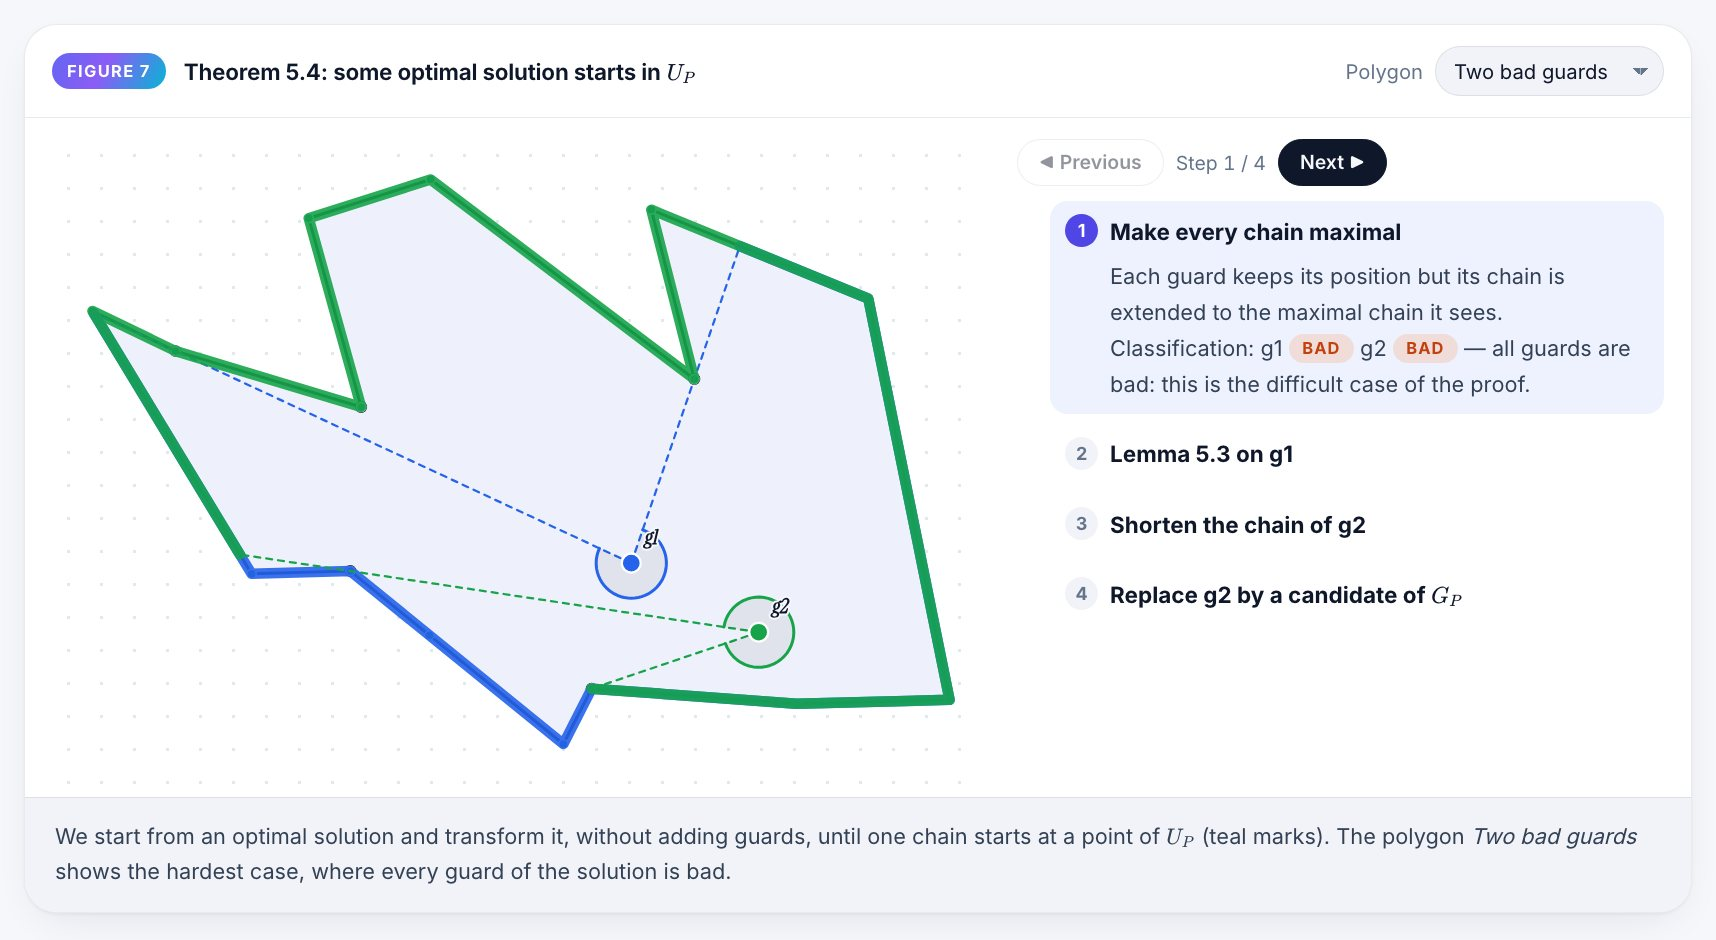
\includegraphics[width=0.8\linewidth]{fig07}
\caption{Figure 7 of our webpage: the proof of Theorem~5.4 applied step by step to an optimal solution made only of bad guards.}
\label{fig:thm54}
\end{figure}

\subsection[Maximal visible chains]{Maximal visible chains \by{Jomaa Abdulrahman}}
\label{sec:lemma62}

For $g\in P$ and $m\in\bd$ seen by $g$, let $E_{g,m}$ be the longest contiguous sequence of edges containing $m$ such that $g$ is to the left of the supporting
line of each of them (Definition~6.1).

\paperthm{lemma}{6.2}
\begin{lemma}
Let $s$ and $t$ be the first and last vertex of a subsequence $E\subseteq E_{g,m}$ with $m\in[s,t]\neq\bd$, let $\pi_s$ and $\pi_t$ be the shortest paths from $s$
and $t$ to $g$, and $r_s$, $r_t$ the rays from $g$ along their last edges. They hit $[s,t]$ in $u$ and $v$, and $[u,v]$ is the unique maximal chain of $[s,t]$
seen by $g$ that contains $m$.
\end{lemma}

\begin{remark}[Our finding]
When the chain $[s,t]$ winds around $g$ more than once, a ray can hit $[s,t]$ twice, and the statement does not say which point to take.
The proof decides it: $u$ is the hit on $[s,m]$ \emph{closest to $m$} (the last point $u^*$ of $[s,m]$ such that $gu^*$ touches $\pi_s$ in more than one point),
and symmetrically for $v$. Our first implementation took the hit closest to $g$ and disagreed with a direct visibility computation in about 19\% of random cases;
with the rule of the proof, it agrees in all our tests. The result of the paper is correct; only the statement needs this precision.
\end{remark}

With the data structures of~\cite{GuibasHershberger1989} and~\cite{HershbergerSuri1995}, the construction costs $O(\log n)$ (Lemma~6.5).

\begin{figure}[ht]
\centering
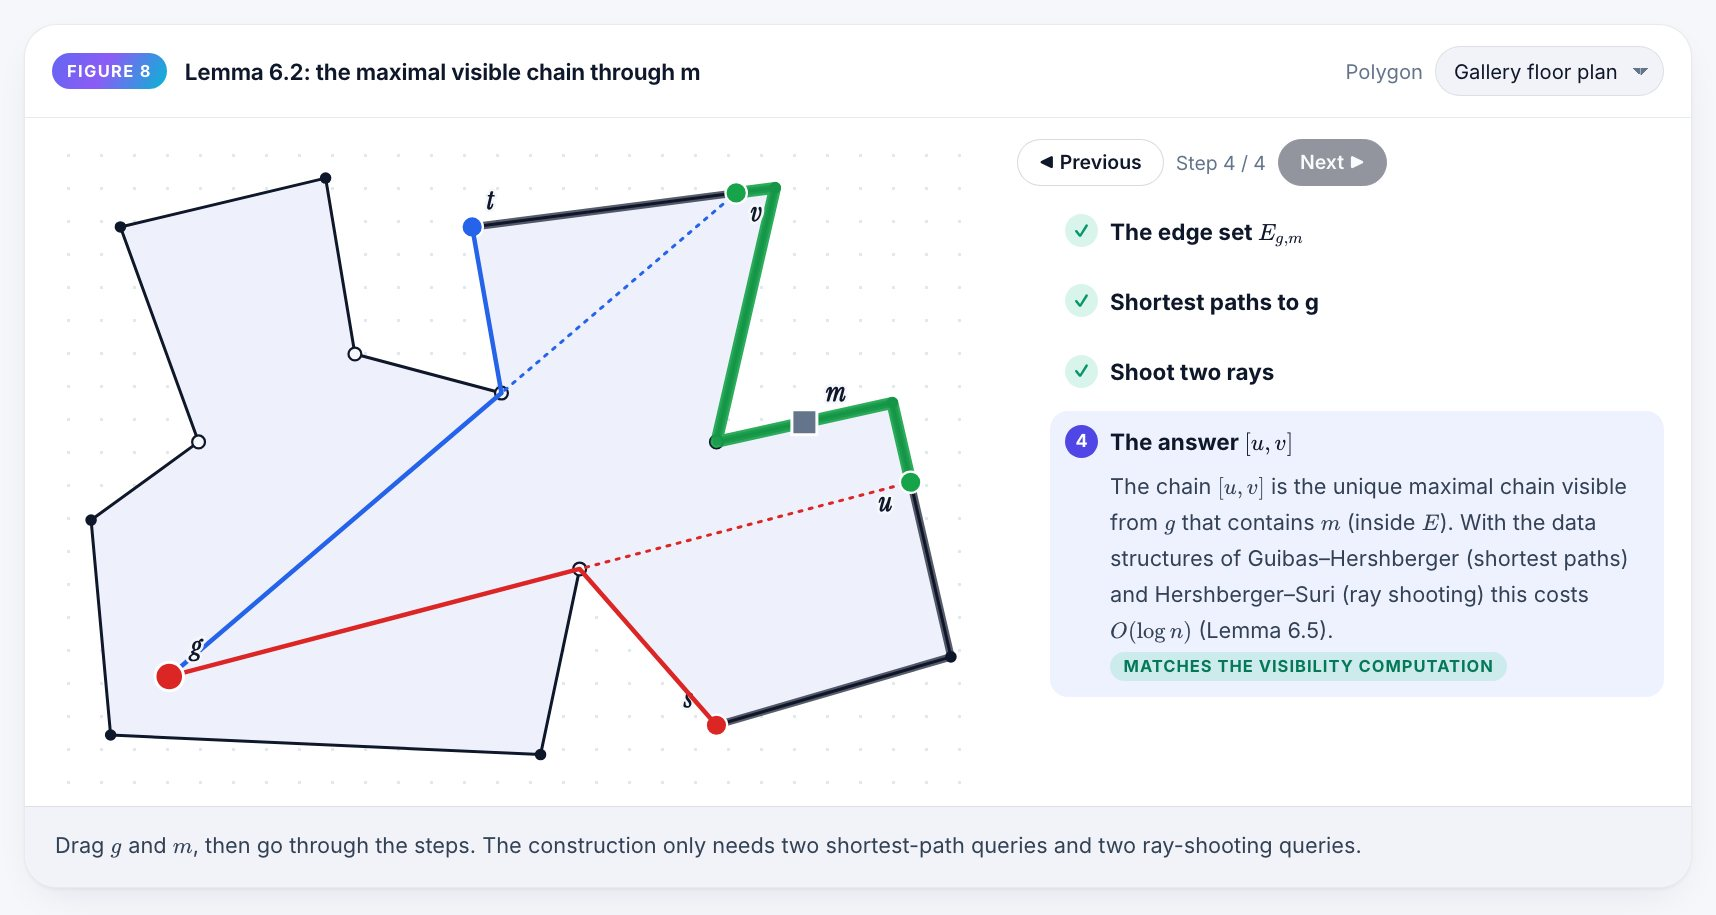
\includegraphics[width=0.8\linewidth]{fig08}
\caption{Figure 8 of our webpage: Lemma~6.2 with the two shortest paths (red and blue), the two rays and the resulting maximal chain $[u,v]$ (green),
checked against a direct visibility computation.}
\label{fig:l62}
\end{figure}

\subsection[One greedy step and the complete algorithm]{One greedy step and the complete algorithm \by{Jomaa Abdulrahman}}

\paperthm{lemma}{6.8}
\begin{lemma}
A simple polygon $P$ can be stored in a data structure in $O(n^2\log n)$ time and $O(n^2)$ space such that, for any $u\in\bd$, $\nextop(u)$
and a guard realising it can be computed in $O(\log^2 n)$ time.
\end{lemma}

The query takes the best candidate guard of $G_P$ whose chain contains $u$ (good guards, by Corollary~4.7), and searches for a bad guard by binary search on
the edge where its chain could end: the shortest path from $u$ must turn left (Observation~4.8), which gives the line $\ell_u$, intersected with the visibility
core, and Lemma~4.9 says that one of the two endpoints of this intersection is as good as the best bad guard.

\paperthm{theorem}{7.1}
\begin{theorem}
The Contiguous Art Gallery Problem can be solved in $O(kn^2\log^2 n)$ time and $O(n^2)$ space: $O(n^2)$ starting points, $O(k)$ greedy steps each, and
$O(\log^2 n)$ time per step.
\end{theorem}

\subsection[\texorpdfstring{Towards the optimal $\Theta(n\log n)$ algorithm}{Towards the optimal Theta(n log n) algorithm}]{Towards the optimal $\Theta(n\log n)$ algorithm \by{Jomaa Abdulrahman}}
\label{sec:optimal}

The follow-up paper~\cite{deBerg2026} reduces the starting points to $O(n)$ with dominating guards, computes $\nextop$ for all starting points at once with a
sliding window, and represents $\nextop$ with $O(n)$ pieces that are constant or M\"obius transformations $x\mapsto\frac{A+Bx}{C+Dx}$, which removes the factor $k$.
A reduction from set disjointness gives a matching $\Omega(n\log n)$ lower bound. We explain these ideas on the webpage but did not implement them.

%======================================================================
\section{Implementation and results}
%======================================================================

\subsection{Architecture}

Everything runs in the browser (JavaScript, React for the interface, Vite for the build, KaTeX for formulas), so the webpage can be hosted on GitHub Pages and
every figure recomputes live when the user moves a point. The geometry code is in \texttt{src/geometry/}:

\begin{center}
\begin{tabularx}{\linewidth}{@{}l Y@{}}
\toprule
File & Content \\
\midrule
\texttt{vec.js}, \texttt{polygon.js} & vectors, orientation test, boundary parameter, visibility test of a segment, simplicity test \\
\texttt{visibility.js} & maximal chains seen by a point \\
\texttt{core.js} & visibility cores (intersection of half-planes) \\
\texttt{shortestPath.js} & shortest paths inside $P$ \\
\texttt{arrangement.js} & vertices of the arrangement $C_P$ inside $P$ \\
\texttt{solver.js} & $G_P$, $U_P$, $\nextop$, the greedy algorithm, the full algorithm \\
\texttt{proofs.js} & the constructions of the proofs, used by the figures and the tests \\
\texttt{generate.js} & random simple polygons for the game \\
\bottomrule
\end{tabularx}
\end{center}

\subsection{Simplifications}

As announced in our proposal, we did not implement the polylogarithmic data structures. Shortest paths are computed on the visibility graph of the vertices
(Floyd--Warshall); the arrangement is computed by intersecting all pairs of supporting lines; the search for bad guards scans the edges after $u$ one by one
instead of a binary search, maintaining the visibility core incrementally and stopping as soon as it becomes empty. The algorithm is the same; only the speed
of the subroutines changes, which is fast enough for polygons with a few dozen vertices. The solver also stops early: if the first greedy run uses $m$ guards,
then $k\ge m-1$, so a run with $m-1$ guards is optimal.

\paragraph{Robustness.} The algorithm constantly uses points that lie exactly on supporting lines and segments that graze reflex vertices. We therefore treat
$P$ as a closed set, test visibility by splitting a segment at all its contacts with the boundary, and use small tolerances. The example polygons are slightly
perturbed so that they are in general position, as assumed in the paper.

\subsection{Validation}

We tested the implementation against independent brute-force computations (\texttt{npm test}):
\begin{itemize}
\item visibility chains agree with direct segment tests on random points;
\item $\nextop(u)$ computed as in Lemma~6.8 is never beaten by a dense grid of candidate guards;
\item the greedy algorithm from 200 evenly spaced starts never finds fewer guards than the $U_P$-based optimum, and never uses more than $k+1$ guards;
\item every construction of the proof was checked on the guards of 60 random polygons (\texttt{node tests/proofs-test.mjs 60}): Proposition~4.3 and Corollary~4.7 produced a valid replacement for
8647 of 8647 good guards, Lemma~4.9 for 1381 of 1381 bad guards, our Lemma~6.2 construction matched the direct visibility computation in 5014 of 5014 cases,
and the walk-through of Theorem~5.4 ended at a point of $U_P$ in 61 of 61 cases.
\end{itemize}
In total, 1541 of 1541 checks pass. On random polygons, the full algorithm takes about 10\,ms for $n=12$, 26\,ms for $n=20$, 121\,ms for $n=30$
and 320\,ms for $n=40$ (Node.js on a laptop).

\subsection{The webpage}

The webpage has a short overview (the support of our presentation), five chapters for the proof, a game and the report. The eleven figures illustrate the
steps of the proof (Table~\ref{tab:widgets}); each one calls the same functions as the solver. In the game, the page generates a random simple polygon, the
player places guards and chooses their chains, and the game checks the solution and compares it with the optimum computed by our solver
(Figure~\ref{fig:game}). After feedback from a fellow student, the animations of the overview play only once, can be replayed, and can be switched off.

\begin{table}[ht]
\centering\small
\begin{tabularx}{\linewidth}{@{}l l Y l@{}}
\toprule
Figure & Section & What it shows & Explained by \\
\midrule
1 & Overview & a contiguous guard, the maximal chains it sees, an optimal solution & Ilias \\
2 & 2.1 & the visibility core of a chain (Observations 2.1, 2.2) & Ilias \\
3 & 2.2 & the greedy algorithm and the $k+1$ bound & Ilias \\
4 & 2.3 & good and bad guards (Definition 4.1) & Ilias \\
5 & 2.4 & replacement of good guards (Corollary 4.7) and bad guards (Lemma 4.9) & Ilias \\
6 & 2.5 & the arrangement, $G_P$ and $U_P$ & Jomaa \\
7 & 2.6 & Theorem 5.4 step by step & Jomaa \\
8 & 2.7 & Lemma 6.2 & Jomaa \\
9 & 2.8 & one greedy step (Lemma 6.8) & Jomaa \\
10 & 2.9 & the complete algorithm (Theorem 7.1) & Jomaa \\
11 & 2.10 & the function $\nextop$, basis of the $\Theta(n\log n)$ algorithm & Jomaa \\
\bottomrule
\end{tabularx}
\caption{The interactive figures of the webpage.}
\label{tab:widgets}
\end{table}

\begin{figure}[ht]
\centering
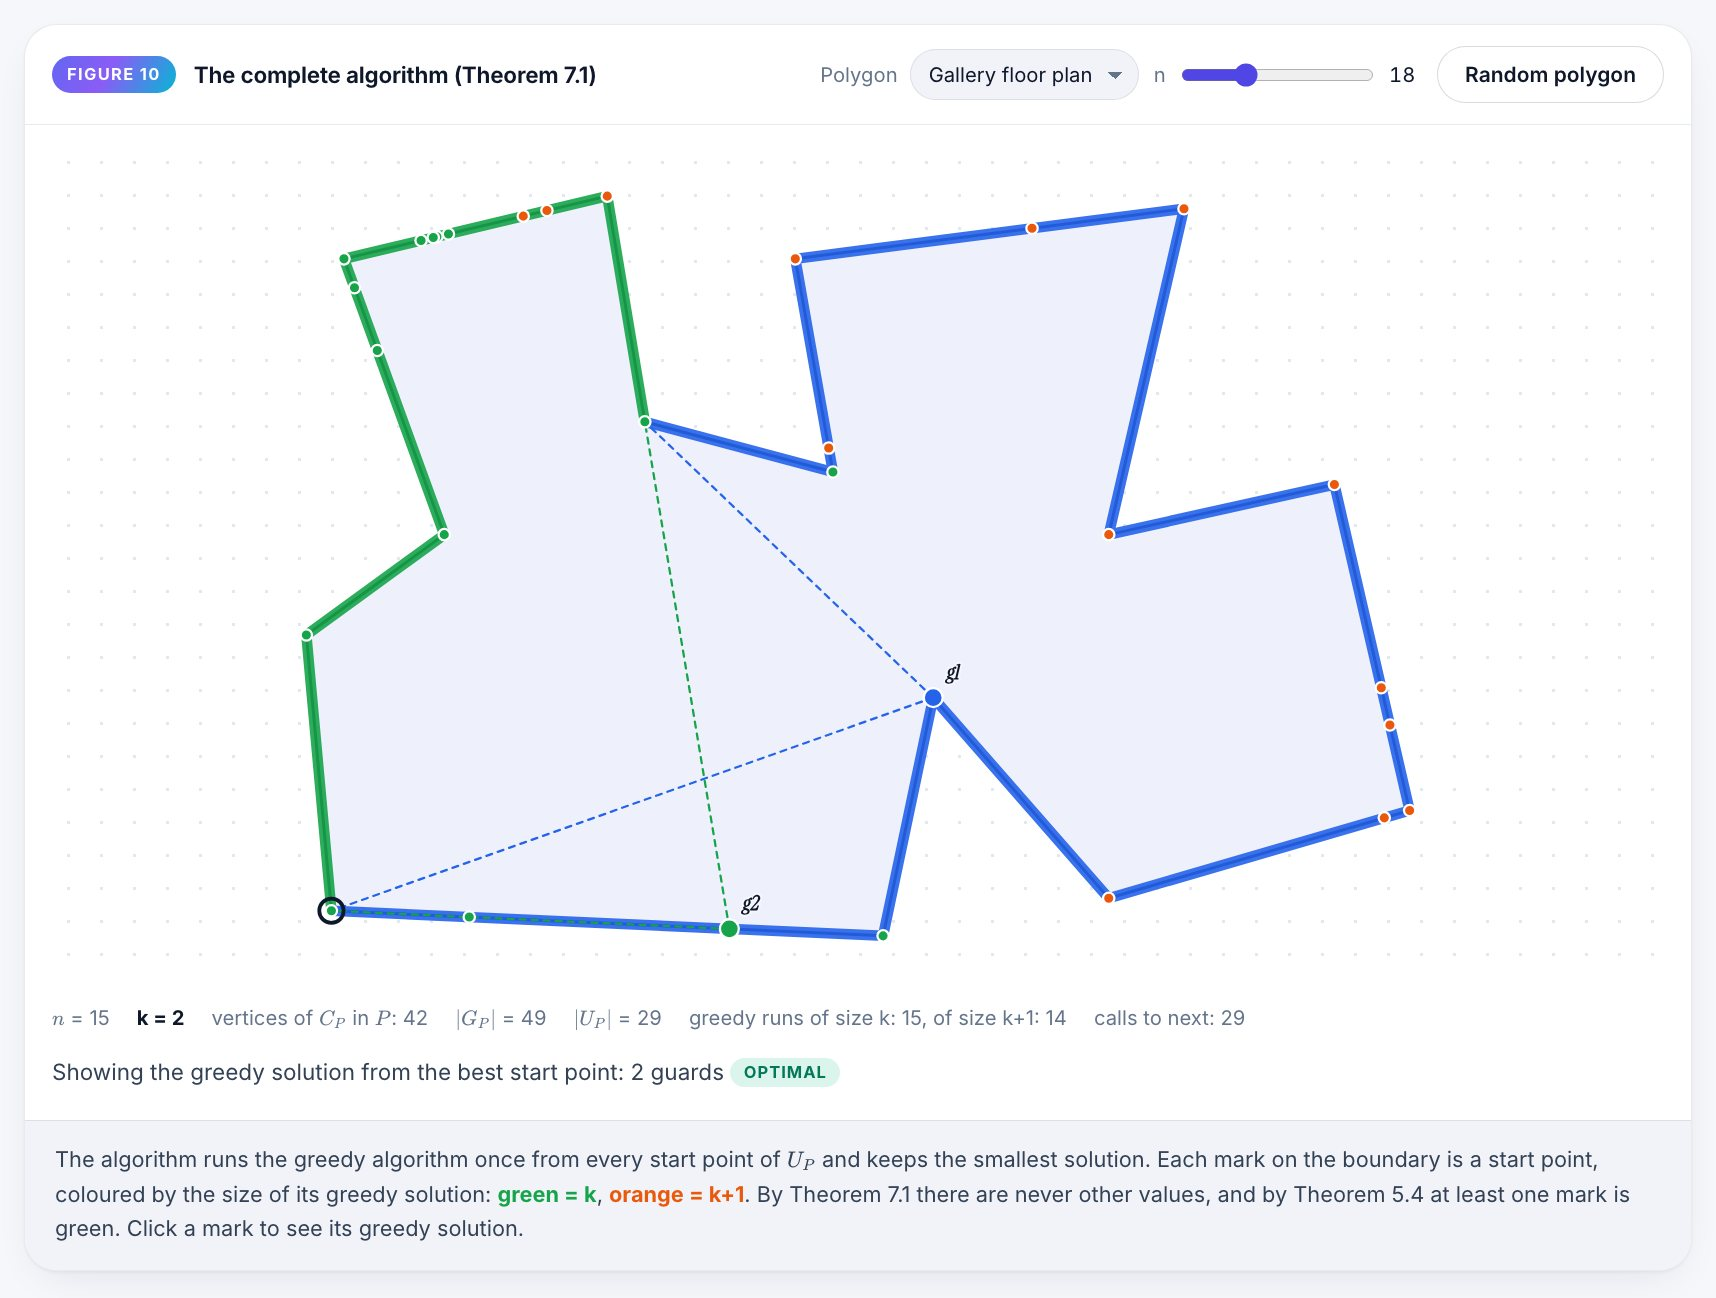
\includegraphics[width=0.48\linewidth]{fig10}\hfill
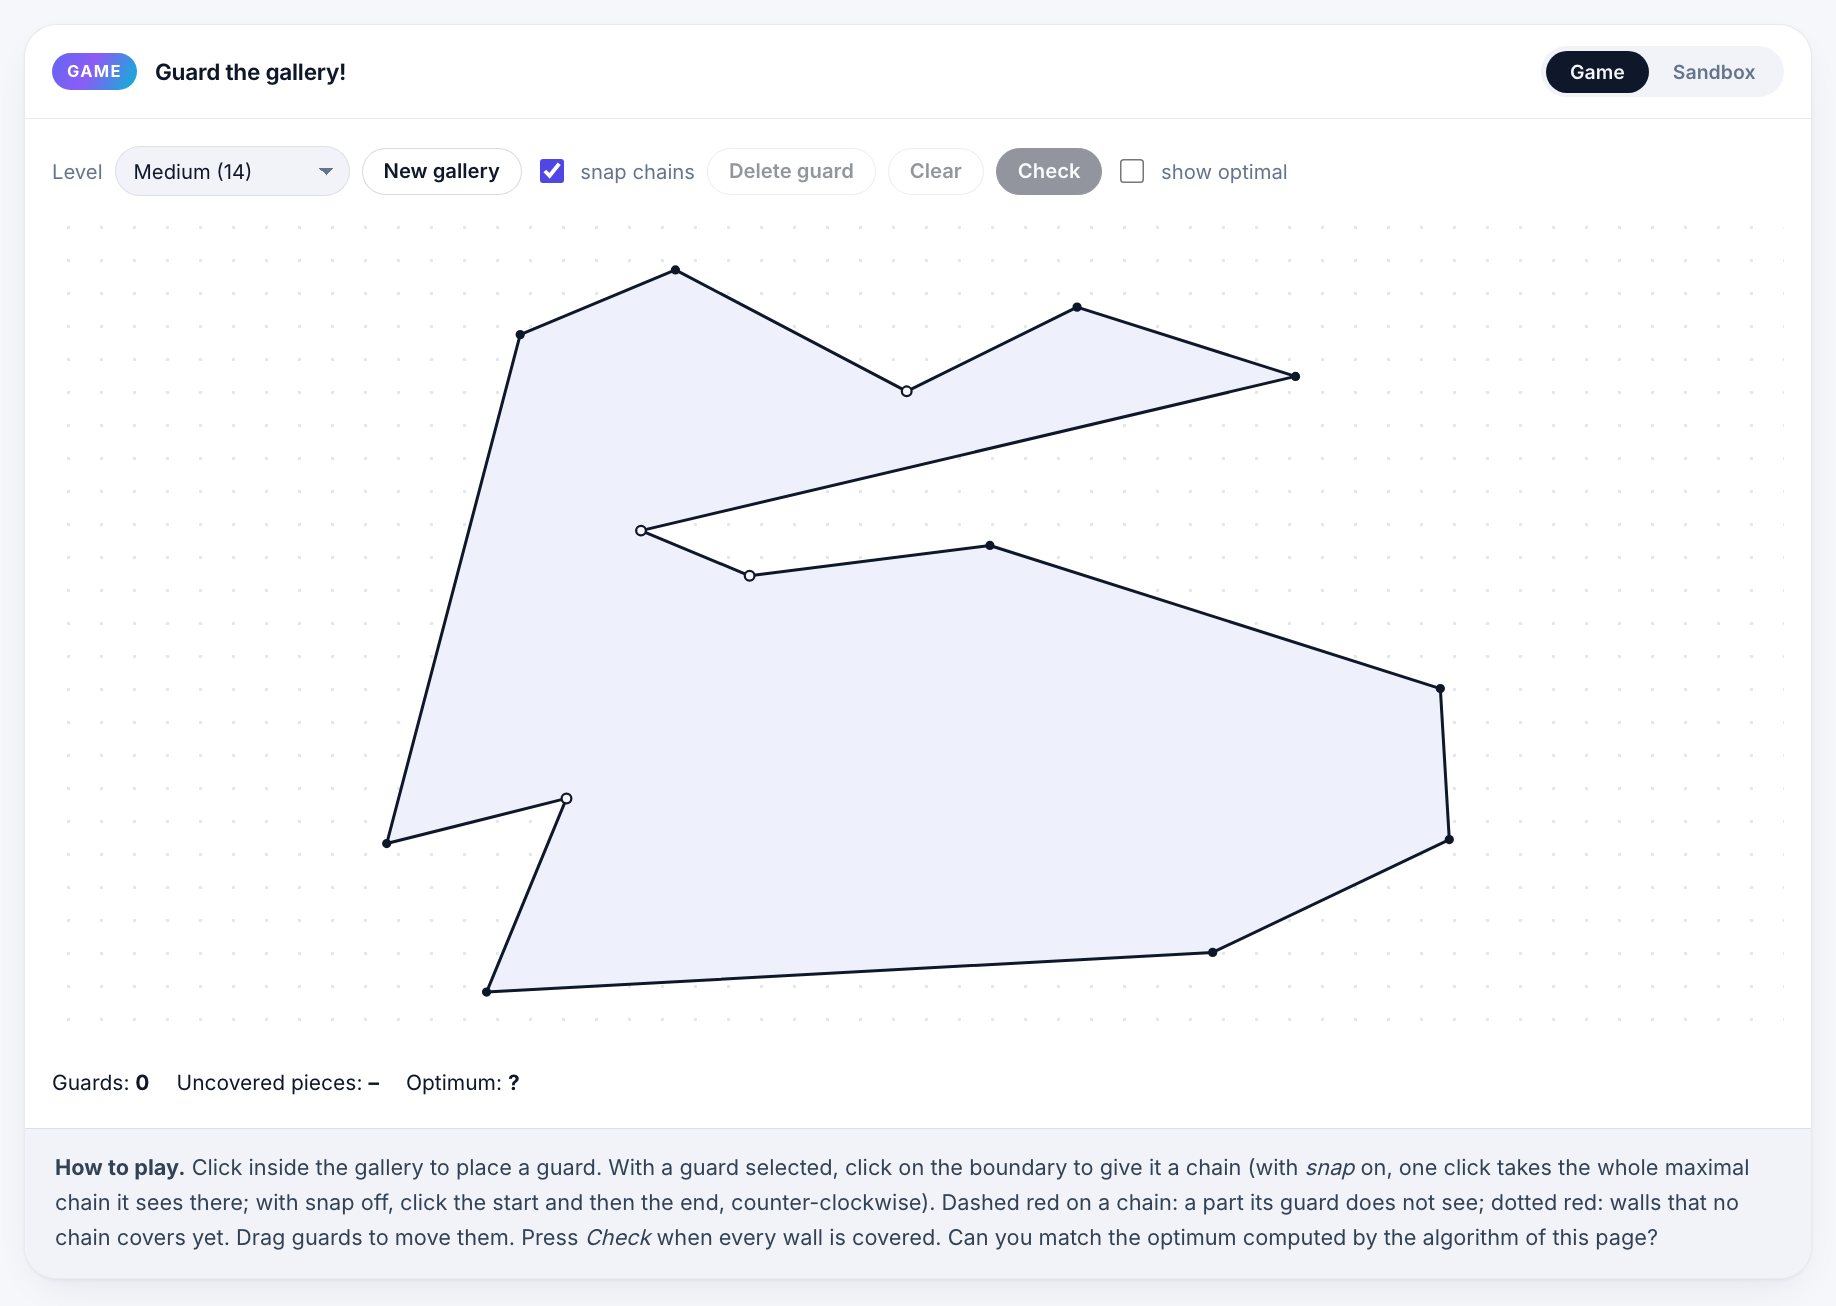
\includegraphics[width=0.48\linewidth]{fig12_game}
\caption{Left: Figure 10 of our webpage, the complete algorithm; every point of $U_P$ is coloured by the size of the greedy solution that starts there
(green $=k$, orange $=k+1$). Right: the game.}
\label{fig:game}
\end{figure}

%======================================================================
\section{Conclusion}
%======================================================================

The Contiguous Art Gallery Problem is a rare art gallery problem that can be solved in polynomial time, because contiguity turns it into covering a
cycle with intervals: once the start of one optimal chain is known, the greedy algorithm is optimal. The paper of de Berg et al.\ shows that $O(n^2)$ starting
points, built from the arrangement of the supporting lines, always contain such a start. Implementing every step of the proof and testing it on random
polygons helped us understand it in detail, and revealed that the statement of Lemma~6.2 needs a precision. The case of polygons with holes remains open.

%======================================================================
\section{Team: who did what}
%======================================================================

\paragraph{Following the feedback on our proposal.} Our proposal had four parts: 1.~the problem, 2.~the algorithm of~\cite{deBerg2025}, 3.~a game, 4.~the report.
It planned that Ilias would work on part~1, Jomaa on part~2, and both on parts~3 and~4. The professor asked us to keep part~1 short, to both work on part~2,
the core of the project, and to split its explanations, with web widgets for the steps of the proof. We did so: part~1 is now a single section of the overview,
and part~2 is split into two halves of the proof, each of us explaining one half, with one interactive widget per step.

\begin{table}[ht]
\centering\small
\begin{tabularx}{\linewidth}{@{}Y l Y l@{}}
\toprule
Step of the proof & Section, widget & Code & Who \\
\midrule
Visibility cores; one guard iff $P$ is star-shaped (Obs.~2.1, 2.2) & 2.1, Fig.~2 & \texttt{core.js}, \texttt{visibility.js} & Ilias \\
The greedy algorithm and the $k+1$ bound & 2.2, Fig.~3 & \texttt{solver.js}: \texttt{next}, \texttt{greedy}, \texttt{solve} & Ilias \\
Good and bad guards (Def.~4.1) & 2.3, Fig.~4 & \texttt{solver.js}: \texttt{classifyGuard} & Ilias \\
Replacing guards (Prop.~4.3, Lem.~4.2--4.6, Cor.~4.7, Lem.~4.9) & 2.4, Fig.~5 & \texttt{proofs.js}: \texttt{replaceGoodGuard}, \texttt{lemma49} & Ilias \\
Arrangement, $G_P$, $U_P$ (Def.~5.1, 5.2, Lem.~5.3) & 2.5, Fig.~6 & \texttt{arrangement.js}; \texttt{solver.js}: \texttt{candidateGuards}, \texttt{startPoints} & Jomaa \\
Theorem 5.4 & 2.6, Fig.~7 & \texttt{proofs.js}: \texttt{theorem54} & Jomaa \\
Maximal visible chain (Lem.~6.2) & 2.7, Fig.~8 & \texttt{shortestPath.js}; \texttt{proofs.js}: \texttt{maximalChainLemma62} & Jomaa \\
One greedy step (Lem.~6.5--6.8) & 2.8, Fig.~9 & \texttt{solver.js}: \texttt{nextBad} & Jomaa \\
Complete algorithm (Thm.~7.1) & 2.9, Fig.~10 & uses \texttt{solve} & Jomaa \\
The $\Theta(n\log n)$ algorithm~\cite{deBerg2026} & 2.10, Fig.~11 & (not implemented) & Jomaa \\
\bottomrule
\end{tabularx}
\caption{Part 2, the algorithm of~\cite{deBerg2025}: who did which step of the proof.}
\label{tab:who}
\end{table}

\begin{table}[ht]
\centering\small
\begin{tabularx}{\linewidth}{@{}l Y Y@{}}
\toprule
Part & Ilias Akajou & Jomaa Abdulrahman \\
\midrule
1. The problem (kept short) & Overview 01--02 and Figure 1 & pointed out that the simple-polygon assumption had to be stated on the overview \\
Geometry basics & \texttt{vec.js}, \texttt{polygon.js} & \\
3. Game and sandbox & \texttt{GameWidget.jsx}, \texttt{generate.js} & \\
Validation & & automatic tests (\texttt{tests/}), overview section 05 \\
4. Report & summary, context & related work, implementation \\
Webpage & structure, design, animations, deployment & review of the webpage \\
Presentation (12 min) & 0:00--5:15 and 11:15--12:00 & 5:15--11:15 \\
\bottomrule
\end{tabularx}
\caption{The other parts.}
\end{table}

\paragraph{Together.} The choice of the topic, the proposal and its revision, the division of the work, the team, acknowledgement and reference sections
of the report, and the AI journal.

\paragraph{How we worked.} The code, the widgets and the first drafts of the texts were produced with an AI assistant, in development sessions led by Ilias
(Section~\ref{sec:ai}). For each part, the person named above checked it against the paper, tested it, and explains it in the presentation.

%======================================================================
\section{Acknowledgements, sources and use of AI}
\label{sec:ai}
%======================================================================

\paragraph{Acknowledgements.} We thank our professor for the feedback on our proposal (keep the classical art gallery problem short, share the explanation
of the algorithm, illustrate the steps of the proof with widgets), and a fellow student for feedback on the course forum about the animations of the overview.

\paragraph{Sources.} All definitions, lemmas and theorems of Section~\ref{sec:algo} are paraphrased from~\cite{deBerg2025} and keep its numbering; Section~\ref{sec:optimal} summarises
\cite{deBerg2026}. All figures are computed by our implementation; no figure was copied from the papers.

\paragraph{Use of AI.} We used an AI assistant (Claude, by Anthropic) to help us understand the papers, to implement and test the code, and to draft the texts
of the webpage and of this report. We reviewed, tested and corrected its results; for example, the wrong choice of ray hit in our first implementation of Lemma~6.2 was found by our tests.
Our AI journal, which describes this use in detail, is provided with the submission.

\paragraph{Software.} React and Vite (MIT licence), KaTeX (MIT), vite-plugin-singlefile (MIT), and the fonts Inter, Instrument Serif and JetBrains Mono
(SIL Open Font License). No other code was reused.

%======================================================================
\begin{thebibliography}{99}
%======================================================================

\bibitem{Biniaz2025}
A.~Biniaz, A.~Maheshwari, M.~C.~R. Merrild, J.~S.~B. Mitchell, S.~Odak, V.~Polishchuk, E.~W. Robson, C.~M. Rysgaard, J.~K.~R. Schou, T.~Shermer,
J.~Spalding-Jamieson, R.~Svenning, D.~W. Zheng.
\newblock Polynomial-time algorithms for contiguous art gallery and related problems.
\newblock In \emph{Proc.\ 41st International Symposium on Computational Geometry (SoCG 2025)}, volume 332 of LIPIcs, pages 20:1--20:21, 2025.
\newblock \href{https://doi.org/10.4230/LIPIcs.SoCG.2025.20}{doi:10.4230/LIPIcs.SoCG.2025.20}.

\bibitem{Merrild2024}
M.~C.~R. Merrild, C.~M. Rysgaard, J.~K.~R. Schou, R.~Svenning.
\newblock The contiguous art gallery problem is solvable in polynomial time.
\newblock \href{https://arxiv.org/abs/2412.13938}{arXiv:2412.13938}, 2024 (v3, 2025). Merged into~\cite{Biniaz2025}; full version.

\bibitem{Biniaz2024}
A.~Biniaz, P.~Bose, A.~Maheshwari, J.~S.~B. Mitchell, S.~Odak, V.~Polishchuk, T.~C. Shermer.
\newblock Contiguous boundary guarding.
\newblock \href{https://arxiv.org/abs/2412.15053}{arXiv:2412.15053}, 2024 (v2, 2025). Merged into~\cite{Biniaz2025}; full version.

\bibitem{Robson2024}
E.~W. Robson, J.~Spalding-Jamieson, D.~W. Zheng.
\newblock The analytic arc cover problem and its applications to contiguous art gallery, polygon separation, and shape carving.
\newblock \href{https://arxiv.org/abs/2412.15567}{arXiv:2412.15567}, 2024 (v2, 2025). Merged into~\cite{Biniaz2025}; full version.

\bibitem{deBerg2025}
S.~de~Berg, J.~Conradi, I.~van~der~Hoog, F.~Staals.
\newblock Simpler and faster contiguous art gallery.
\newblock \href{https://arxiv.org/abs/2508.09734}{arXiv:2508.09734}, 2025.

\bibitem{deBerg2026}
S.~de~Berg, J.~Conradi, I.~van~der~Hoog, E.~Rotenberg.
\newblock The contiguous art gallery problem is in $\Theta(n\log n)$.
\newblock \href{https://arxiv.org/abs/2511.02960}{arXiv:2511.02960}, 2025 (v6, 2026).

\bibitem{Chvatal1975}
V.~Chv\'atal.
\newblock A combinatorial theorem in plane geometry.
\newblock \emph{Journal of Combinatorial Theory, Series B}, 18(1):39--41, 1975.
\newblock \href{https://doi.org/10.1016/0095-8956(75)90061-1}{doi:10.1016/0095-8956(75)90061-1}.

\bibitem{LeeLin1986}
D.~T. Lee, A.~K. Lin.
\newblock Computational complexity of art gallery problems.
\newblock \emph{IEEE Transactions on Information Theory}, 32(2):276--282, 1986.
\newblock \href{https://doi.org/10.1109/TIT.1986.1057165}{doi:10.1109/TIT.1986.1057165}.

\bibitem{Abrahamsen2022}
M.~Abrahamsen, A.~Adamaszek, T.~Miltzow.
\newblock The art gallery problem is $\exists\mathbb{R}$-complete.
\newblock \emph{Journal of the ACM}, 69(1):4:1--4:70, 2022.
\newblock \href{https://doi.org/10.1145/3486220}{doi:10.1145/3486220}.
\newblock Preliminary version in STOC 2018. Open access: \href{https://arxiv.org/abs/1704.06969}{arXiv:1704.06969}.

\bibitem{Stade2025}
J.~Stade.
\newblock The point-boundary art gallery problem is $\exists\mathbb{R}$-hard.
\newblock In \emph{Proc.\ 41st International Symposium on Computational Geometry (SoCG 2025)}, volume 332 of LIPIcs, pages 74:1--74:23, 2025.
\newblock \href{https://doi.org/10.4230/LIPIcs.SoCG.2025.74}{doi:10.4230/LIPIcs.SoCG.2025.74}.

\bibitem{GuibasHershberger1989}
L.~J. Guibas, J.~Hershberger.
\newblock Optimal shortest path queries in a simple polygon.
\newblock \emph{Journal of Computer and System Sciences}, 39(2):126--152, 1989.
\newblock \href{https://doi.org/10.1016/0022-0000(89)90041-X}{doi:10.1016/0022-0000(89)90041-X}.

\bibitem{Guibas1987}
L.~J. Guibas, J.~Hershberger, D.~Leven, M.~Sharir, R.~E. Tarjan.
\newblock Linear-time algorithms for visibility and shortest path problems inside triangulated simple polygons.
\newblock \emph{Algorithmica}, 2:209--233, 1987.
\newblock \href{https://doi.org/10.1007/BF01840360}{doi:10.1007/BF01840360}.

\bibitem{LeePreparata1979}
D.~T. Lee, F.~P. Preparata.
\newblock An optimal algorithm for finding the kernel of a polygon.
\newblock \emph{Journal of the ACM}, 26(3):415--421, 1979.
\newblock \href{https://doi.org/10.1145/322139.322142}{doi:10.1145/322139.322142}.

\bibitem{HershbergerSuri1995}
J.~Hershberger, S.~Suri.
\newblock A pedestrian approach to ray shooting: shoot a ray, take a walk.
\newblock \emph{Journal of Algorithms}, 18(3):403--431, 1995.
\newblock \href{https://doi.org/10.1006/jagm.1995.1017}{doi:10.1006/jagm.1995.1017}.
\newblock Preliminary version in \emph{Proc.\ 4th ACM-SIAM Symposium on Discrete Algorithms (SODA 1993)}, 54--63.

\end{thebibliography}

\end{document}
